\section{Episode 49: Madness Reigns - In the Hall of the Mountain King}

\begin{multicols}{2}

\DndDropCapLine{R}ip blows a massive hole win the wall with his new weapon. Epic!. As the room shakes and parts of the ceiling starts to rain down us, I feel a dark presence closing in on us. Before I can say anything a huge part of the building starts crashing down around us. This is the inherent danger of not living in a hovel! At any moment you could be squished by the building itself! The giant mountain lizard, has come to say hello. Myron doesn’t seem as keen as I expected.\medskip

The ceiling makes its second appearance of the night, we manage to crawl out, but where the fuck has Burnie gone! “This is our cue to go” aren’t exactly the best epitaph, but sometimes that how it goes. Well there is no time like the present to waste looking for characters. Perhaps I could call on the big lizard guy to help us out. Everything is too heavy around here, why do people live underneath such big bits of stone! Riphard finds Burnies limp hand, probably not for the first time. Exmeh finds the door, but it seems stuck. I unstuck it with a mercury fulminate arrow, its pretty effective. Myron and Riphard drag out a bedraggled looking Burnie. Proof if ever it was needed of the danger or living in a massive palace tower.\medskip

I provide some options for the party, Myron is not happy with the giant lizard, and deems the giant sink hole as a bad option too. I think this is going to be the best, “Fucking Goblins always want to get in the shit” Riphard rudely states to Myron. “Its good for you Riphard, thats why they always put it on plants” Exmerahs elegant repost. Exmerah gets nothing but warbled static and mentions of a giant lizard from Delilah. Seems like good news to me. Yes yes, I say I jump backwards down into the hole, only to hit the wall hard. It was particularly painful. But seems like we are taking my second favourite plan. Obviously the first would be much more effective, especially when it came to smiting our enemies. But sewers it is I guess.\medskip

These are some pretty high quality sewers, if I was a sewer inspector, then I would be pretty impressed. Myrons natural instinct identifies that we should follow the flow of shit. I check with out latest iteration of Boss, and his lordship says no more scouting shinanigans for old lord olok. Its not so much that I’m in a huff, just I want to make sure nothing sneaks up on us….. Burnie is the master of turd spotting, perhaps it was a part of the book burner training. Martha certainly liked to use to add flavour to stews… We have a brief discussion about what happened to the cows, Myron. “Of course the cows, got away” says I only to be rebuffed by BossMan Big pants. The huge pile of shit in the middle of the room erupts and two shit covered ugly as frog/toad creatures emerge. “Jabba it inthe butt” classic Exmerah. \medskip

“Looks like its wednesday my dudes” Riphard says before unloading the hammer of the gods into one of them. Boom time toady mother crunchers. A beam of light is thrown from the pistol, lighting the room up, and filling it with the smell of acrid burning flesh. Exmerah blasts one, Stanri jumps on it, I take the knee and let fly a little arrow. Burnie ducks and rolls out of the way of one mega toady, and points back at him. Somehow this helps me realise I should shoot this one. As he is doing this he is narrowly missed by a giant slathering tongue. Getting eaten by one of these would be pretty unpleasant. The other toad turns on its belly and encases Stanri in its giant freaking mouth. Thats going to be hard to digest. Myron eyes up the giant beast, and then goes in with the pacifier. Very stabby. Rip quick switches his weapons and unloads a shell straight into one of the toads. It sinks in with a dull thud, as the toads skin crumples under the ballistic pressure.\medskip

Exmerah makes the first attempt to free Stanri, turns out shooting it really helped Stanri to get out of its mouth. As I knock and unload into the one burnie was shouting at. His dark highness then mimics my action and shoots the same fat toad. Again screaming at me to shoot it. A toad suddenly dissappears, only to reappear behind Exmerah, who luckily spots it in the shiny armour of Stanri, and manages to dodge its darting bite. Myron has had enough, and “fucking bursts it” one toad down. Exmerah and Rip then blow the last mega toad to pieces. The toads stomach is slapped open, and he spills his guts across the sewer.\medskip

Burnies broken gloves have clearly upset Exmerah, sometimes I think he is really rude, other times I see a shy broken child that never learnt to play with others. Either way his gloves won’t be working for a little while. Exmerah gets Stanri to ping, and he opens to give out a large coil of metal. He now has a beef jerky flavoured snare, could be pretty good. She then feeds Stanri a healing potion, for someone so smart she probably should have realised it wouldn’t work on a mechanical beast. Its time to go up and face the world. It becomes clear from Myrons postulating that the possible death of the cows, clearly has hit him worse than I had previously thought. “I’m not sure if it can fly, but I am sure it can bleed”. “If it can bleed, then we can kill it”. Classic Gabrin talk \medskip

We emerge to a city that is collapsing in on itself. The armies are within the walls, and cutting down the enemy in swathes. The mega GoJira is still here, thank whatever gods really exist. The casual swing of its tail is knocking out a whole villages worth of city. This thing is what I wish I dreamed of being. Instead of that weird jungle slug.. Delilah has thankfully taken the skyship out of range and is circling from a large distance. So far I wonder how we will get up there. The cows are nowhere to be seen. But Myron seems to have a great plan…. We are going to mount the beast and run up it. The group don’t seem so sure that its a great idea, so instead we call in on Delilah.\medskip

While ship wheels around, the dark presence is upon me again. We are getting bum rushed by all kinds of different people. Thankfully I recognise our ninja robot friends, less fortunately is a large red robed figure hovering in his own darkness above us. He is flanked by some church wardens. This could get nice and ugly pretty quickly, maybe I should have taken some health potions after all… The inquisitor warns us that we should have not come, it is time for some serious levels of deception. I reply in kind to the inquisitor “Yes Master”, although to be honest I barely convince myself (nat 1 deception (-1)). Rip gets the end game off with a bang, flashing a cosmic beam of light straight through the Iniquisitor. Sweet goblin jesus, it looks like it actually hurt the bastard. Time to hide near Riphard. Burnie gets made into a pin cushion by the archers, as the heart thrust society starts swaning in, time for some sexy mecha ninja carnage.\medskip

Myron takes stock of the situation, before planting a kiss on Exmerahs head, who whisper back to “be brilliant”. God they are the darndest cutest couple. She slaps a forcefield on me, and then melts back in a blur of movement. Somehow we will survive this, just as we survived all the others. Things look like they are going to be ok, until the the inquisitor sends long streaks of lightening from his fingers, frying Exmerah, Riphard, Burnie and I to a fine crispy finish. That has got to be one of the most painful things that has ever happened to me. Burnie the brave mother fucker, takes front and center and pulls the fire of the arbiters fire. God dam sometimes for someone with the psyche of a mal adjusted child, I can really see what Martha saw in him. Maybe its just the recent bowt of lightening coursing through my veins but as he stands there in the open still smoking from his own dose of high voltage he looks ever inch the hero.\medskip

I step back behind the statue for cover and try to thin the crowd of attackers. I definetely hit that archer, but its to little avail as the “possibly friendly” Lizard stomps down on the house and building annihilating the poor poor person. Maybe he is on our team? The battle rages on around us, I have to say war has never been so much fun. Not really it is absolutely horrifying, no wonder people came back different in the Varg. Myron circles around the foot, then leaps majestically plunging his bayonet into the creatures foot. Is it time to climb onto our beast?? Could it be….Exmerah tosses me a potion, and seems to be onboard with Myrons climbing plan. The inquisitor clicks his fingers and...Riphard snaps out of existence at the same time. This is going to be problematic. Burnie rushes back to see wtf happened to Riphard. I run to his aid, shoot a line into the monster to hook myself and Burnie in. At this point Delilah comes swooping in, and blows a cannon ball straight into the house behind the Inquisitor. The guy visible flinches as it all comes tumbling down behind him. At which point a beacon of light appears next to Burnie.\medskip

Myron holds on for dear life, clutching the his precious cargo of Exmerah close to his bosom. The leg has lifted, and is carrying them away as the he lets slip Exmerah. I asked one thing of him, and perhaps it was too much. She is falling perhaps to her doom, when Stanri launches to a few rockets at her, these latch onto her legs and she sticks the hard three point land. Crushing the pacing below her. Sweet jesus what a cool little bitch she has become.\medskip

“What have you done, you have touched that which must not be harmed” Echoes through our minds, probably from the freaky scary guy. As his words cut through me, and his red glowing eyes come towards me. Its as if his voice has unlocked a part of me long forgotten, and I stand, no dangle 50 ft below the big friendly lizards frozen. Chaos ensues around me, but still I can feel his presence seeping deeper into me. I know nothing but the cold presence of fear. `following records not witnessed by kolo the unwise`. The airship comes swooping down again, unleashing a ballista. Rubrix entices us to board again as it sweeps underneath the beast to retrieve us. As rope drops, from the airship, Rip wraps it around one arm, and lets fly another beam of radiant light right through the side of his body.\medskip

As I come to I notice that everyone is milling around below us, I notice the ship and Rubrix standing on it beckoning to us all. Myron is hanging on for dear life above me, and below me is an ongoing war. I can’t believe the airship has come so dam close to the foot. This is some kind of ace sky pilot of the future surely. Exmerah pulls out the cube and runs toward the Hearthrust team and Stanri, strangely nothing seems to happen. The inquisitor floats across the square finger outreached at Exmerah, a dark shadow rips forth from his finger and encompases my sister. She collapses under the strain of his evil energies. Burnie bless his soul, once again plays the hero running to her aid. Stanris reaction is a class act too, as he rains hell down upon the the inquisitor.\medskip

I come around and shoot another roped arrow into the airship. I have successfully attached the monster to the airship. Nothing could go wrong, except I am unable to dislodge the arrow from the monster. As the monster lifts its foot, over the airship Myrons leaps down, and rolls out of the fall. So many hero moves today. Riphard tucks the rope under him, and while dangling from the airship levels the hammer of the gods at the Inquisitor a beam of searing light blasts forth into the evil man. Half of his body is blown away and an empty corpse falls lifeless to the ground. Team hearthrust grab the others and run for the rope, literally saving everyone bacon.\medskip

Myron blast the rope attaching me to the monster to pieces, letting me swing free. This is really not what I had in mind, but it was Myrons plan… Stanri rushes past to the rope scooping up the inquisitor. And clamping his jaws on the end of the rope. I have some stern words with Myron, about the dropping of my sister. “Hello boys, I think we have a bit of a monster lizard problem to solve” she says as she jumps over the side of the ship. Myron strides over to her and swings her in his arms.\medskip

Burnie appears with a set of cocktails, what a man! Myron unleashes the smoke machine, Delilah screams, and a spout of flame engulfs the entire ship. The purple flames envelop the ship, catching Myron and Burnie unaware. At which point a field of magical energy, surrounds the ship protecting it. Rubrix is giving his last to save us. “You must escape” and a large claw comes down to smite the airship, Rubrix bleeds from his nose and lets be honest a few other areas as well. He holds us close, and imparts the last gem of wisdoms to us “The best lessons are ones learnt by yourself” . He floats off the back of the airship into the air itself. He envelops the monsters claw with a field of raw energy only he could manifest. “You must get back to Velterra” are his genuine epitaph, which isn’t bad to be honest, considering a giant lizard totally destroyed him.\medskip

We sail of into the unknown once more. We also return to check on the the charred corpses of our comrades, who fortunately have not died. We rip his talons off his hands, and find a bankers note 1500 gp. We also find a note:\medskip

“These pawns must be stopped, Lazarus people are getting too close to success, Signed Kylon” Also has a spiky spiral symbol on it. I give it to you for one second and you break it” - Rip says as myron watches the letters disappear on the note paper. Myron peels back the mask, and reveals a mostly human face, except for a tentacled maw. “I’m sure the church can bleed too” says Exmerah as she ties the corpse to the front of the ship.\medskip

He dropped her\medskip

fade out to https://www.youtube.com/watch?v=zf2aIVKp1OY\medskip

\end{multicols}

\vspace*{5mm}

\begin{center}
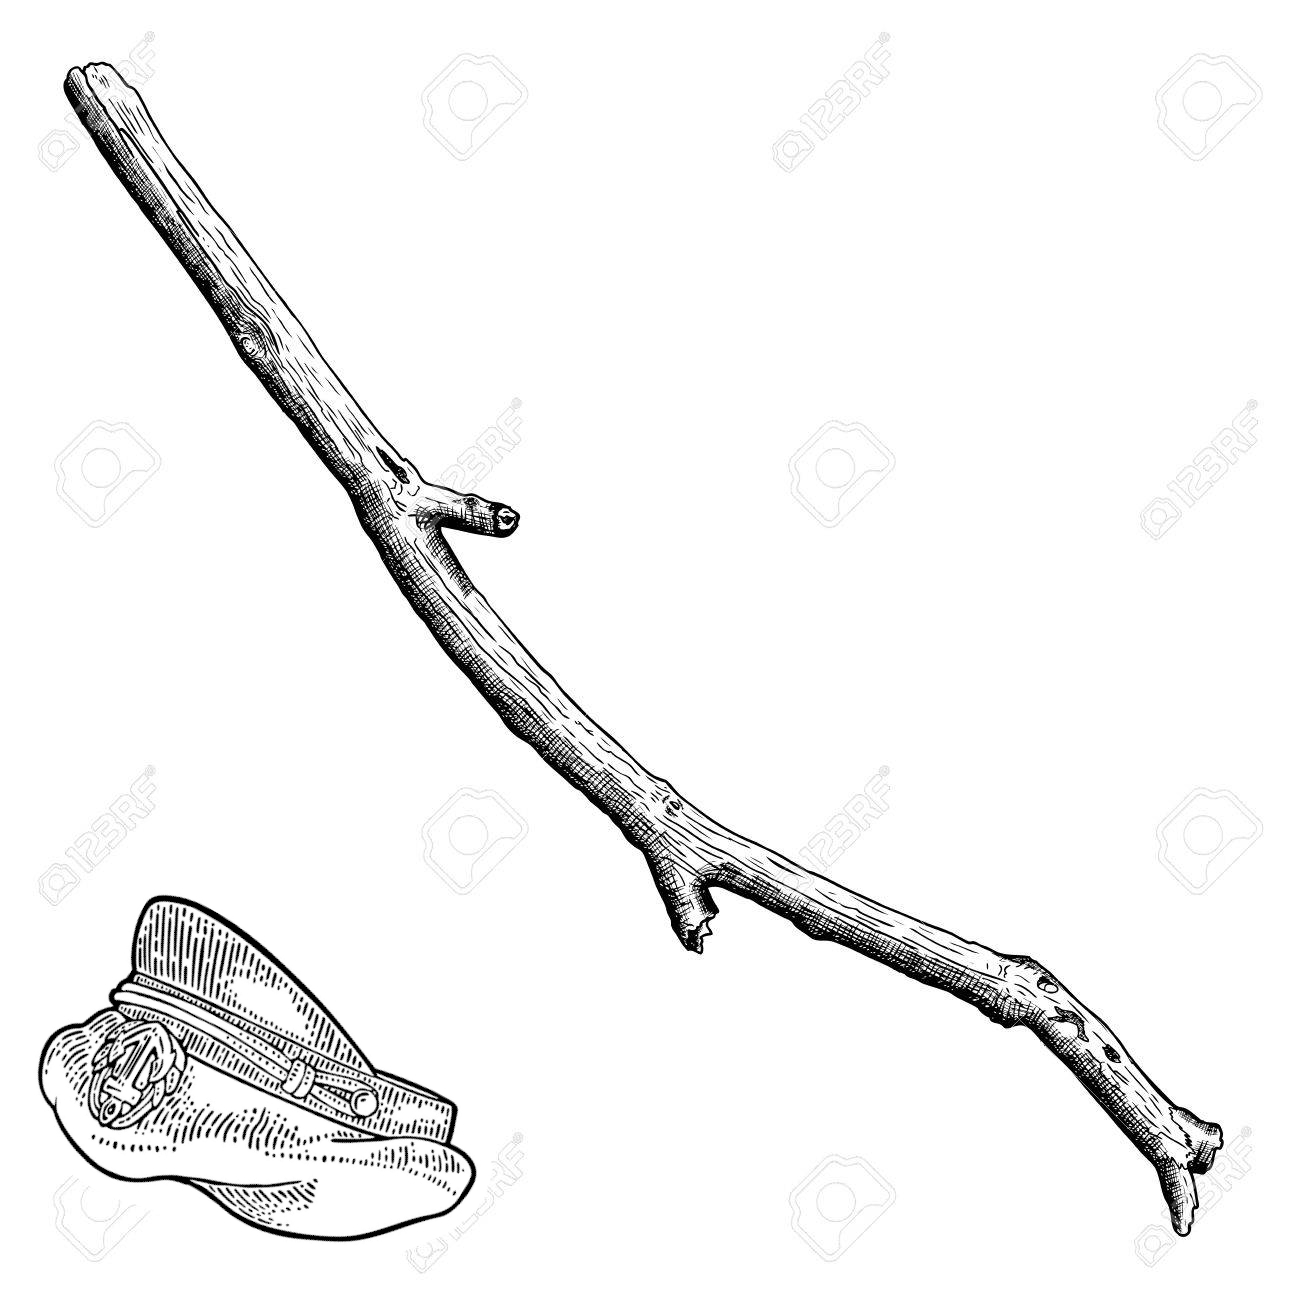
\includegraphics[width=\textwidth]{./content/img/xxx.jpg}
\begin{figure}[h]
\end{figure}
\end{center}

\clearpage